\documentclass[a4paper,5pt]{amsbook}
%%%%%%%%%%%%%%%%%%%%%%%%%%%%%%%%%%%%%%%%%%%%%%%%%%%%%%%%%%%%%%%%%%%%%

\usepackage{booktabs}
\usepackage{graphicx}
\usepackage{multicol}
\usepackage{textcomp}
\usepackage{systeme}
\usepackage{amssymb}
\usepackage[]{amsmath}
\usepackage{subcaption}
\usepackage[inline]{enumitem}
\usepackage{gensymb}

%%%%%%%%%%%%%%%%%%%%%%%%%%%%%%%%%%%%%%%%%%%%%%%%%%%%%%%%%%%%%%

\newcommand{\sen}{\,\mbox{sen}}
\newcommand{\tg}{\,\mbox{tg}\,}
\newcommand{\cosec}{\,\mbox{cosec}\,}
\newcommand{\cotg}{\,\mbox{cotg}\,}
\newcommand{\tr}{\,\mbox{tr}\,}
\newcommand{\ds}{\displaystyle}
\newcommand{\ra}{\rightarrow}

%%%%%%%%%%%%%%%%%%%%%%%%%%%%%%%%%%%%%%%%%%%%%%%%%%%%%%%%%%%%%%%%%%%%%%%%

\setlength{\textwidth}{16cm} \setlength{\topmargin}{-1.7cm}
\setlength{\textheight}{25cm}
\setlength{\leftmargin}{1.2cm} \setlength{\rightmargin}{1.2cm}
\setlength{\oddsidemargin}{0cm}\setlength{\evensidemargin}{0cm}

%%%%%%%%%%%%%%%%%%%%%%%%%%%%%%%%%%%%%%%%%%%%%%%%%%%%%%%%%%%%%%%%%%%%%%%%

% \renewcommand{\baselinestretch}{1.6}
% \renewcommand{\thefootnote}{\fnsymbol{footnote}}
% \renewcommand{\theequation}{\thesection.\arabic{equation}}
% \setlength{\voffset}{-50pt}
% \numberwithin{equation}{chapter}

%%%%%%%%%%%%%%%%%%%%%%%%%%%%%%%%%%%%%%%%%%%%%%%%%%%%%%%%%%%%%%%%%%%%%%%

\begin{document}
\thispagestyle{empty}
\pagestyle{empty}
\begin{minipage}[h]{0.14\textwidth}
	
\includegraphics[scale=0.24]{../ufgd.png}
\end{minipage}
\begin{minipage}[h]{\textwidth}
\begin{tabular}{c}
{{\bf UNIVERSIDADE FEDERAL DA GRANDE DOURADOS}}\\
{{\bf C\'alculo Diferencial e Integral --- Lista 6}}\\
{{\bf Prof.\ Adriano Barbosa}}\\
\end{tabular}
\vspace{-0.45cm}
%
\end{minipage}

%------------------------

\vspace{1cm}
%%%%%%%%%%%%%%%%%%%%%%%%%%%%%%%%   formulario  inicio  %%%%%%%%%%%%%%%%%%%%%%%%%%%%%%%%
\begin{enumerate}
    \vspace{0.5cm}
    \item Encontre a equa\c{c}\~ao da reta tangente as curvas abaixo nos pontos
        dados:

        \noindent{}
        \begin{enumerate*}
            \item $y=4x-3x^2$, $(2,-4)$
            \hspace{1cm}
            \hspace{1cm}
            \item $y=\sqrt{x}$, $(1,1)$
        \end{enumerate*}

    \vspace{0.5cm}
    \item O deslocamento retil\'{\i}neo de uma part\'{\i}cula \'e dado pela equa\c{c}\~ao
        $s(t)=\ds\frac{1}{t^2}$. Determine a velocidade da part\'{\i}cula nos
        instantes $t=1$, $t=2$ e $t=a$ com $a$ um n\'umero real positivo
        qualquer.

    \vspace{0.5cm}
    \item Use o gr\'afico de $f$ abaixo para estimar o valor das derivadas:

        \noindent{}
        \begin{enumerate*}
            \item $f'(-3)$
            \hspace{0.5cm}
            \hspace{0.5cm}
            \item $f'(-2)$
            \hspace{0.5cm}
            \hspace{0.5cm}
            \item $f'(-1)$
            \hspace{0.5cm}
            \hspace{0.5cm}
            \item $f'(0)$
            \hspace{0.5cm}
            \hspace{0.5cm}
            \item $f'(1)$
            \hspace{0.5cm}
            \hspace{0.5cm}
            \item $f'(2)$
            \hspace{0.5cm}
            \hspace{0.5cm}
            \item $f'(3)$
        \end{enumerate*}

        \begin{figure}[h]
            \centering
            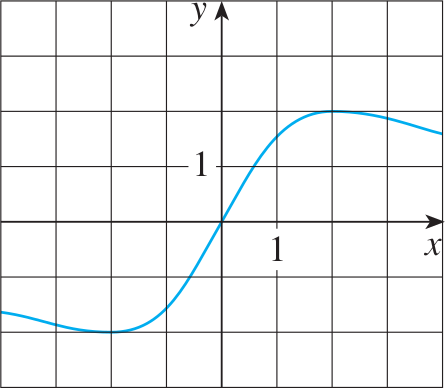
\includegraphics[width=0.25\textwidth]{lista-06-fig1.png}
        \end{figure}

    \vspace{0.5cm}
    \item Determine os pontos onde as fun\c{c}\~oes abaixo n\~ao s\~ao deriv\'aveis.
        \begin{figure}[h]
            \centering
            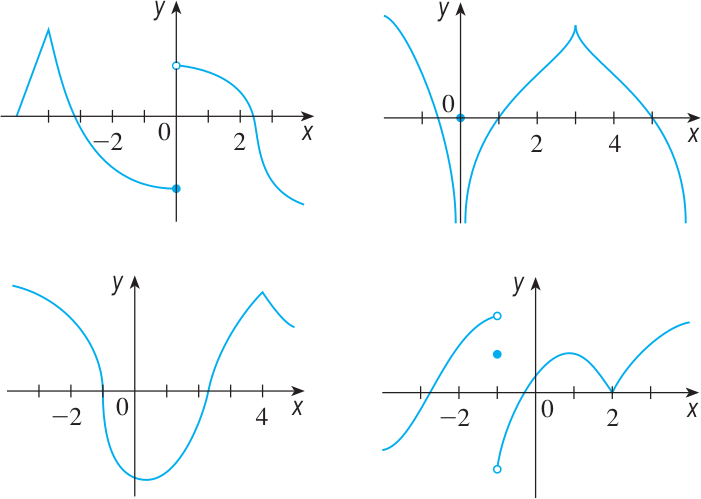
\includegraphics[width=0.5\textwidth]{lista-06-fig2.png}
        \end{figure}

    \newpage{}
    \vspace{0.5cm}
    \item Use as regras de deriva\c{c}\~ao para calcular a derivada das fun\c{c}\~oes
        abaixo.
        \begin{figure}[h]
            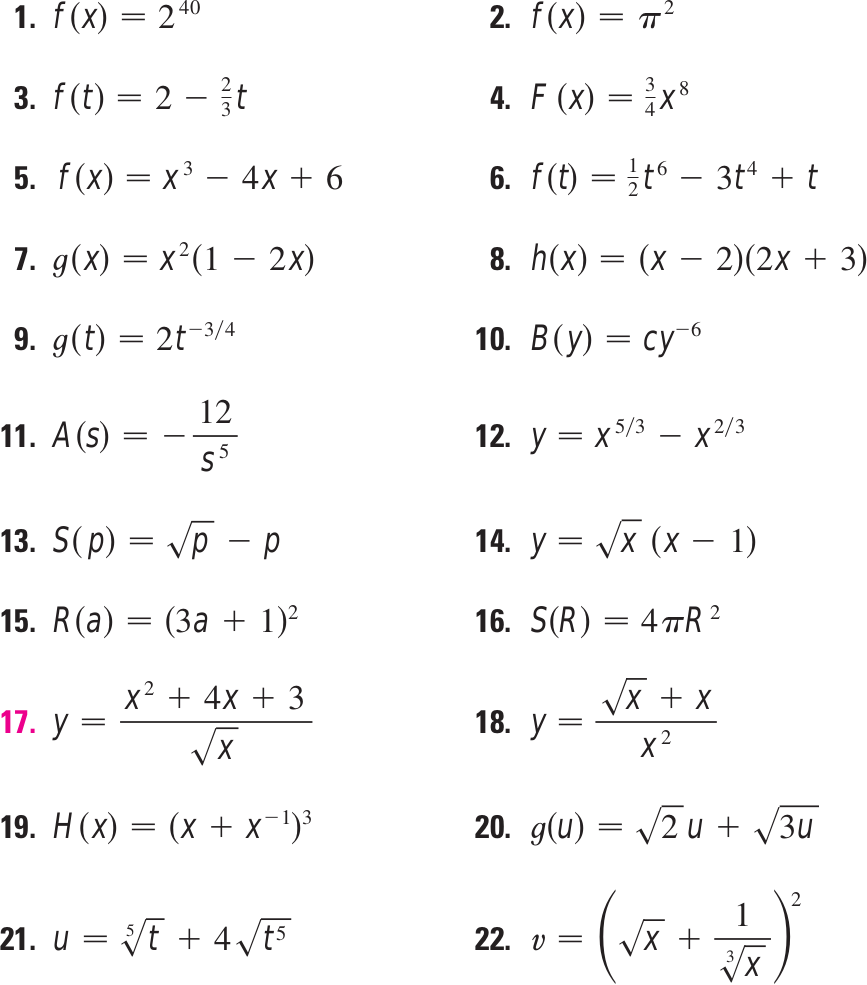
\includegraphics[width=0.6\textwidth]{lista-06-fig3.png}
        \end{figure}
\end{enumerate}

\end{document}
